%%
%% This is file `sample-lualatex.tex',
%% generated with the docstrip utility.
%%
%% The original source files were:
%%
%% samples.dtx  (with options: `sigconf')
%% 
%% IMPORTANT NOTICE:
%% 
%% For the copyright see the source file.
%% 
%% Any modified versions of this file must be renamed
%% with new filenames distinct from sample-lualatex.tex.
%% 
%% For distribution of the original source see the terms
%% for copying and modification in the file samples.dtx.
%% 
%% This generated file may be distributed as long as the
%% original source files, as listed above, are part of the
%% same distribution. (The sources need not necessarily be
%% in the same archive or directory.)
%%
%%
%% Commands for TeXCount
%TC:macro \cite [option:text,text]
%TC:macro \citep [option:text,text]
%TC:macro \citet [option:text,text]
%TC:envir table 0 1
%TC:envir table* 0 1
%TC:envir tabular [ignore] word
%TC:envir displaymath 0 word
%TC:envir math 0 word
%TC:envir comment 0 0
%%
%%
%% The first command in your LaTeX source must be the \documentclass
%% command.
%%
%% For submission and review of your manuscript please change the
%% command to \documentclass[manuscript, screen, review]{acmart}.
%%
%% When submitting camera ready or to TAPS, please change the command
%% to \documentclass[sigconf]{acmart} or whichever template is required
%% for your publication.
%%
%%
\documentclass[sigconf]{acmart}
\usepackage{hyperref}
\usepackage{graphicx}
\usepackage{geometry}
%\usepackage{float}
\geometry{a4paper}
%\citestyle{acmauthoryear}

%%
%% \BibTeX command to typeset BibTeX logo in the docs
\AtBeginDocument{%
  \providecommand\BibTeX{{%
    \normalfont B\kern-0.5em{\scshape i\kern-0.25em b}\kern-0.8em\TeX}}}

%% Rights management information.  This information is sent to you
%% when you complete the rights form.  These commands have SAMPLE
%% values in them; it is your responsibility as an author to replace
%% the commands and values with those provided to you when you
%% complete the rights form.
\setcopyright{rightsretained}
\copyrightyear{2022}
%\acmYear{2018}
\acmDOI{}

%% These commands are for a PROCEEDINGS abstract or paper.
\acmConference[Information Society 2021]{Information Society 2021: 24th international multiconference}{4--8 October 2021}{Ljubljana, Slovenia}
%%
%%  Uncomment \acmBooktitle if the title of the proceedings is different
%%  from ``Proceedings of ...''!
%%
%%\acmBooktitle{Woodstock '18: ACM Symposium on Neural Gaze Detection,
%%  June 03--05, 2018, Woodstock, NY}
\acmPrice{}
\acmISBN{}
\settopmatter{printccs=false, printacmref=false}


%%
%% Submission ID.
%% Use this when submitting an article to a sponsored event. You'll
%% receive a unique submission ID from the organizers
%% of the event, and this ID should be used as the parameter to this command.
%%\acmSubmissionID{123-A56-BU3}

%%
%% For managing citations, it is recommended to use bibliography
%% files in BibTeX format.
%%
%% You can then either use BibTeX with the ACM-Reference-Format style,
%% or BibLaTeX with the acmnumeric or acmauthoryear sytles, that include
%% support for advanced citation of software artefact from the
%% biblatex-software package, also separately available on CTAN.
%%
%% Look at the sample-*-biblatex.tex files for templates showcasing
%% the biblatex styles.
%%

%%
%% The majority of ACM publications use numbered citations and
%% references.  The command \citestyle{authoryear} switches to the
%% "author year" style.
%%
%% If you are preparing content for an event
%% sponsored by ACM SIGGRAPH, you must use the "author year" style of
%% citations and references.
%% Uncommenting
%% the next command will enable that style.
%%\citestyle{acmauthoryear}


%%
%% end of the preamble, start of the body of the document source.
\begin{document}

%%
%% The "title" command has an optional parameter,
%% allowing the author to define a "short title" to be used in page headers.
\title{Analysis of Transfer Learning for Named Entity Recognition in South-Slavic Languages}

%%
%% The "author" command and its associated commands are used to define
%% the authors and their affiliations.
%% Of note is the shared affiliation of the first two authors, and the
%% "authornote" and "authornotemark" commands
%% used to denote shared contribution to the research.
\author{Nikola Ivačič}
%\authornote{Both authors contributed equally to this research.}
\email{nikola.ivacic@gmail.com}
%\orcid{1234-5678-9012}
%\author{G.K.M. Tobin}
%\authornotemark[1]
%\email{webmaster@marysville-ohio.com}
\affiliation{%
  \institution{Jožef Stefan Institute\\
  Jamova cesta 39}
  \streetaddress{Jamova cesta 39}
  \city{Ljubljana}
  \country{Slovenia}
  \postcode{1000}
}

\author{Hanh Tran}
\affiliation{%
  \institution{Jožef Stefan Institute\\
  Jamova cesta 39}
  \streetaddress{Jamova cesta 39}
  \city{Ljubljana}
  \country{Slovenia}
  \postcode{1000}}

\author{Boshko Koloski}
\affiliation{%
  \institution{Jožef Stefan Institute\\
  Jamova cesta 39}
  \streetaddress{Jamova cesta 39}
  \city{Ljubljana}
  \country{Slovenia}
  \postcode{1000}
}

\author{Senja Pollak}
\affiliation{%
 \institution{Jožef Stefan Institute\\
  Jamova cesta 39}
  \streetaddress{Jamova cesta 39}
  \city{Ljubljana}
  \country{Slovenia}
  \postcode{1000}}

\author{Marko Pranjić}
\affiliation{%
  \institution{Jožef Stefan Institute\\
  Jamova cesta 39}
  \streetaddress{Jamova cesta 39}
  \city{Ljubljana}
  \country{Slovenia}
  \postcode{1000}}

\author{Matthew Purver}
\affiliation{%
  \institution{School of Electronic Engineering and Computer Science\\
  Queen Mary University of London}
  \streetaddress{Mile End Road\\
   London E1 4NS, UK}
  \city{London}
  \country{UK}}

\author{Nada Lavrač}
\affiliation{%
  \institution{Jožef Stefan Institute\\
  Jamova cesta 39}
  \streetaddress{Jamova cesta 39}
  \city{Ljubljana}
  \country{Slovenia}
  \postcode{1000}}

%%
%% By default, the full list of authors will be used in the page
%% headers. Often, this list is too long, and will overlap
%% other information printed in the page headers. This command allows
%% the author to define a more concise list
%% of authors' names for this purpose.
\renewcommand{\shortauthors}{Ivačič et al.}

%%
%% The abstract is a short summary of the work to be presented in the
%% article.
\begin{abstract}
  This paper presents analysis of Named Entity Recognition task for South-Slavic languages using pre-trained multilingual neural network models.
  Observing the performance metrics from prior research showed, that performance of fine-tuned multilingual neural models is very close to the performance of monolingual neural models.
  This observation lead us to a question, that this paper aims to answer: Can fine-tuning of a multilingual pre-trained embeddings with other than the target language corpora improve named entity recognition for a specific language?
\end{abstract}

%%
%% Keywords. The author(s) should pick words that accurately describe
%% the work being presented. Separate the keywords with commas.
\keywords{natural language processing, named entity recognition, neural networks, text tagging, text classification, multilingual pre-trained models}
%% A "teaser" image appears between the author and affiliation
%% information and the body of the document, and typically spans the
%% page.
%% NikComm\begin{teaserfigure}
%% NikComm  \includegraphics[width=\textwidth]{sampleteaser}
%% NikComm  \caption{Seattle Mariners at Spring Training, 2010.}
%% NikComm  \Description{Enjoying the baseball game from the third-base
%% NikComm  seats. Ichiro Suzuki preparing to bat.}
%% NikComm  \label{fig:teaser}
%% NikComm\end{teaserfigure}


%%
%% This command processes the author and affiliation and title
%% information and builds the first part of the formatted document.
\maketitle

\section{Introduction}
Using of multilingual neural models simplifies scalability and applications where many languages are needed for the task.
Therefore getting the performance of a multilingual neural model as close as possible to the performance of a monolinugual one is very beneficial.
Named Entity Recognition (NER) is also one of the corner stones of the Natural Language Processing (NPL) tasks in many text processing systems.
We observed two prior works:
\begin{itemize}
\item BSNLP: 3rd Shared Task on SlavNER\cite{piskorski-etal-2021-slav} submitted paper by Prelevikj and Žitnik et al.\cite{prelevikj-zitnik-2021-multilingual}
\item Clipping industry project developed by Department of Knowledge Technologies at Jožef Stefan Institute\cite{KTIJS}
\end{itemize}
Prior work has shown that the monolingual NER model performance for Slovene language is practically equal to the performance of a multilingual one.
Clipping industry project multilingual model was fine-tuned with other language corpora from the same - South-Slavic family.

The question that naturally arises and this paper tries to answer is this: Did the fine-tuning with related languages influence the performance of a multilingual model?
The problem with comparison of both prior work is that the:
\begin{itemize}
\item corpus preprocessing
\item pre-trained models
\item hyper-parameters
\item performance measures
\end{itemize}
were not strictly the same in both experiments so, one has to be really cautious when evaluating the performance metrics or deriving conclusions from it.
\section{Data Description}
For each language the most commonly used and as many as possible NER corpora was gathered (~\ref{tab:corpora}).
\begin{table}[H]
  \caption{List of Used Corpora}
  \label{tab:corpora}
  \begin{tabular}{llrrl}
    \toprule
    Lang.&Abbr.&Sentences&Tokens&Name\\
    \midrule
    sl&bsnlp&18106&400291&BSNLP 2017/21\cite{piskorski-etal-2021-slav}\\
    sl&500k&9483&193611&ssj500k 2.3\cite{ssj500k-23}\\
    sl&ewsd&2024&31233&{ELEXIS}-{WSD} 1.0\cite{ELEXIS-WSD-10}\\
    sl&scr&18139&391526&{SentiCoref} 1.0\cite{SentiCoref-10}\\
    \midrule
    hr&bsnlp&820&18704&BSNLP 2017 and 2021\cite{piskorski-etal-2021-slav}\\
    hr&500k&820&18704&hr500k 1.0\cite{hr500k-10}\\
    \midrule
    sr&set&3891&86726&{SETimes}.{SR} 1.0\cite{SETimes-SR-1.0}\\
    \midrule
    bs&wann&8917&199378&WikiANN - PAN-X\cite{rahimi-etal-2019-massively}\\
    \midrule
    mk&wann&16227&156467&WikiANN - PAN-X\cite{rahimi-etal-2019-massively}\\
  \bottomrule
  \end{tabular}
\end{table}
CoNLL-2003 shared task\cite{CoNLL2003} NER tags in IOB2\cite{IOB2} format were used as a common denominator for all corpora and experiments.
Each corpus was first combined if split, then converted to common format, reshuffled and split to train / dev / test set in a 80 / 10 / 10 ratio.

When the combined corpora was used we concatenated the sets without further reshuffling so, that the experiments can be repeated.
%Prepared and converted data is available on Github for convenience and possible manual review (move to online resources?).
\subsection{Used corpora}
Table ~\ref{tab:corpora} summarizes used corpora in experiments.

We combined all corpora for each language to further conduct our experiments.
The Slovene corpora was obtained from newly published combined Training corpus {SUK} 1.0\cite{SUK-1.0}
\subsection{Data Conversion}
First obstacle we had to overcome is different tagging of NER corpora.
Here we decided to keep only common tags.
For example: BSNLP corpus uses PRO and EVT tags while WikiANN corpus is missing a MISC tag that is common to ssj500k and hr500k corpora.
All non-common tags, including MISC, were replaced with O (outside IOB) tag except the PER, LOC and ORG tags.

Second obstacle was the difference in format.
BSNLP, for instance, is such corpus that uses separate files for verbatim text and NER tags with no positional reference between one another.
To solve this problem we used CLASSLA\cite{ljubesic-dobrovoljc-2019-neural} sentence segmentation and tokenization and custom conversion.

The third step was to remove sentences longer than 128 tokens and convert corpora from common CoNLL format to CSV format with two fields:
\begin{itemize}
  \item sentence: whitespace separated sentence word tokens.
  \item NER: white space separated NER tags for each sentence word token.
\end{itemize}

The final step was to split the corpus data to train, test, dev sets.

\subsection{Corpora analysis}
Comparing the corpora showed the differences that could potentially be problematic for obtaining aligned model performance, especially considering the NER tag ratios.
In this sense the WikiANN automatically annotated corpora structure was standing out.
\begin{table}[H]
  \caption{Analysis of Used Corpora}
  \label{tab:corpora_analysis}
  \begin{tabular}{lrrrrr}
    \toprule
    lang&tok. / sent.&NER / tok.&PER&LOC&ORG\\
    \midrule
    sl&21.29&9.09\%&31.70\%&22.20\%&34.13\%\\
    hr&20.43&7.41\%&28.71\%&20.55\%&30.82\%\\
    sr&22.29&12.01\%&29.96\%&30.12\%&32.35\%\\
    bs&7.81&36.91\%&31.65\%&29.67\%&38.67\%\\
    mk&9.64&28.07\%&34.89\%&30.32\%&34.79\%\\
    \bottomrule
    \multicolumn{6}{c}{PER, LOC and ORG are ratios with respect to NER}
  \end{tabular}
\end{table}

\begin{figure}[h]
  \centering
  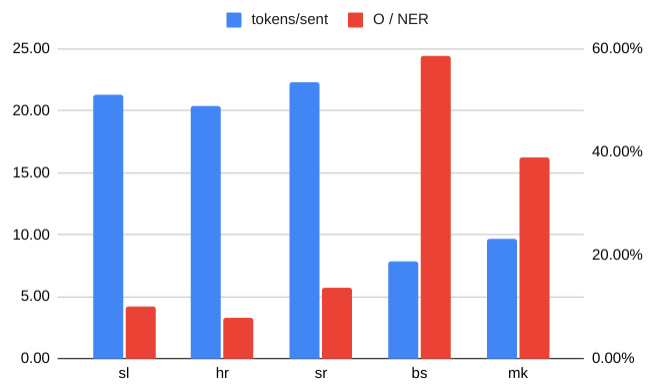
\includegraphics[width=\linewidth]{wikiann-skew}
  \caption{WikiANN corpus skew}
\end{figure}

Fortunately we were unable to detect any inconsistencies regarding performance measurements.

\section{Methods}
For all experiments Hugging Face's transformers Python library\cite{wolf-etal-2020-transformers} was used.
Initial baseline model tests has shown that XLM-RoBERTa (base sized model)\cite{DBLP:journals/corr/abs-1911-02116} consistently outperforms BERT multilingual base model (cased)\cite{DBLP:journals/corr/abs-1810-04805}.
Therefore, due to task and resource limitations, we continued with our experiments using only XLM-RoBERTa base sized pre-trained model.

(TABLE)

The selected method was to first develop a baseline models for each language and produce NER classification measurements.
In the next steps we combined additional remaining language corpora, re-train the model and measure performance changes.

%Czech language was also used, because it is not as closely related as other languages to Slovene and could give us additional insights in possible performance changes.

(TABLE)



Following hyper-parameters were used for all model fine-tuning:
\begin{itemize}
  \item 256 max-length for tokenizer
  \item Pytorch's AdamW algorithm with 5e-5 learning rate
  \item 40 epochs
  \item
\end{itemize}

\section{Evaluation}


\section{Conclusion}

%%
%% The acknowledgments section is defined using the "acks" environment
%% (and NOT an unnumbered section). This ensures the proper
%% identification of the section in the article metadata, and the
%% consistent spelling of the heading.
\begin{acks}
To Robert, for the bagels and explaining CMYK and color spaces.
\end{acks}

%%
%% The next two lines define the bibliography style to be used, and
%% the bibliography file.
\bibliographystyle{ACM-Reference-Format}
\bibliography{atlner}


%%
%% If your work has an appendix, this is the place to put it.
\appendix

\section{Research Methods}

\subsection{Part One}

Lorem ipsum dolor sit amet, consectetur adipiscing elit. Morbi
malesuada, quam in pulvinar varius, metus nunc fermentum urna, id
sollicitudin purus odio sit amet enim. Aliquam ullamcorper eu ipsum
vel mollis. Curabitur quis dictum nisl. Phasellus vel semper risus, et
lacinia dolor. Integer ultricies commodo sem nec semper.

\subsection{Part Two}

Etiam commodo feugiat nisl pulvinar pellentesque. Etiam auctor sodales
ligula, non varius nibh pulvinar semper. Suspendisse nec lectus non
ipsum convallis congue hendrerit vitae sapien. Donec at laoreet
eros. Vivamus non purus placerat, scelerisque diam eu, cursus
ante. Etiam aliquam tortor auctor efficitur mattis.

\section{Online Resources}

Nam id fermentum dui. Suspendisse sagittis tortor a nulla mollis, in
pulvinar ex pretium. Sed interdum orci quis metus euismod, et sagittis
enim maximus. Vestibulum gravida massa ut felis suscipit
congue. Quisque mattis elit a risus ultrices commodo venenatis eget
dui. Etiam sagittis eleifend elementum.

Nam interdum magna at lectus dignissim, ac dignissim lorem
rhoncus. Maecenas eu arcu ac neque placerat aliquam. Nunc pulvinar
massa et mattis lacinia.

\end{document}
\endinput
%%
%% End of file `sample-lualatex.tex'.
